% File name: Tube Challenge/Report/Report.tex
% Report detailing the project etc
% Author: adh
% Date: Tue 02 Jul 2013 16:29

\documentclass[a4paper,11pt]{article}  % Standard document class
\usepackage[english]{babel}            % Set document language
\usepackage{fullpage}                  % Set up page for small margins etc

\usepackage{graphicx}                  % For including images in document
\usepackage{placeins}                  % Allows use of \FloatBarrier
% to avoid images or tables
% moving into next section
\usepackage{subfig}                    % For subfigures...

\usepackage{amsmath}                   % For improving maths/formula typesetting
\usepackage{tabularx}                  % Table changing package

\usepackage{algpseudocode}             % For producing algorithms/flowcharts
\usepackage{listings}                  % For including source code in document

\usepackage{todonotes}

% Provide command for scientific notation
\providecommand{\e}[1]{\ensuremath{\times10^{#1}}}
\providecommand{\degrees}{\ensuremath{^{\circ}}}

% Define title here:
\title{Tube Challenge 2013\\Project Overview}
\author{James Griffith \and Andy Holt \and Chris Murkin \and Dominic
  Newman \and Jack Robinson}
\date{June - August 2013}

\begin{document}

\listoftodos

% generate title
\maketitle

\section*{Overview}

Since he was a young boy, James Griffith has dreamed of visiting every
Tube station in London in a single day. Now, at the age of 21, he's
hoping to make this dream a reality. But he doesn't just want to visit
every station in a day, he's planing to break the world record by
visiting every station, using only public transport and on foot, in
the fastest time ever.

The London Underground is the world's oldest underground
railway. Opening in 1863, and now comprising $402\,\mathrm{km}$ of
track, the Tube forms a vast network of underground tunnels and
carries over a billion passengers per year through London. 2013 marks
the 150$^{\mathrm{th}}$ year of operation of the Underground, and is a
fitting time to attempt the challenge.

The challenge is simple: to visit all 270 stations on the Tube network
in a single day. To beat the record, he needs to do it in
under 16 hours, 29 minutes and 13 seconds.

But being simple by no means makes the challenge easy. With such a
complex transport network and so many passengers, delays are
inevitable and unpredictable. A delay of just a few minutes in the
chosen route could render the whole challenge unachievable due to
missed trains and connections. The physical element of the challenge
is also gruelling: equivalent to running a marathon through busy
London stations, up and down thousands of steps and sprinting to make
fast connections. Another significant issue is shear boredom: over 16
hours of sitting on Tubes in a day will almost certainly make James
want to quit; taking a good book will be of utmost importance.

\section*{The Challenge}

The Tube Challenge is an established contest, first run in March
1960. The official rules have been refined over the years and the
record has been broken many times. The Tube has changed considerably
during this time, causing the record to be reset on multiple
occasions.

The rules as they stand state that:
\begin{itemize}
\item The participant need not travel along every line of the tube,
  but must pass through every station in the network.
  \item Only public transport -- such as train (underground or
    overground) and bus -- and foot may be used. Private transport,
    including cars and bicycles, may not be used.
\end{itemize}

\section*{The Team} \todo{expand/improve bios}

With such a huge task ahead of him, James has enlisted the support of
some friends. \todo{briefly mention cardboard boat team}

\bigskip

\noindent \begin{minipage}{0.4\textwidth}
  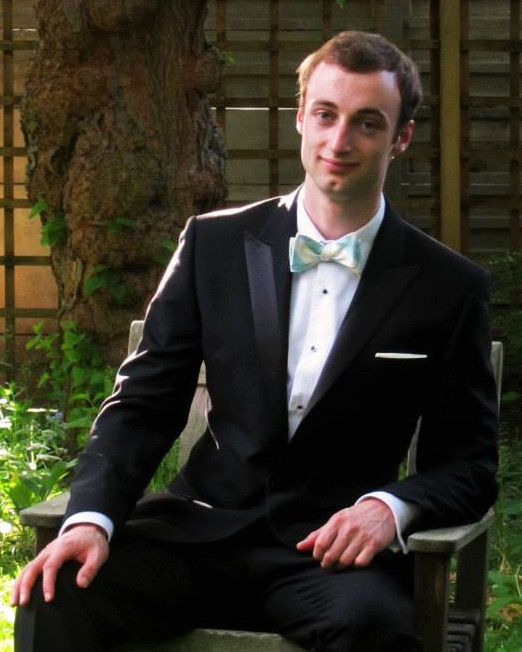
\includegraphics[width=0.8\textwidth]{JamesProfile.jpg}
\end{minipage}
\hfill
\begin{minipage}{0.6\textwidth}
  {\large \textbf{\underline{James Griffith}}}\\

  James is the driving force behind the tube challenge, and he will be
  the one who actually visits the tube stations. James is well suited
  to the task: representing Cambridge in 400m athletics makes him
  ideal for running through and between stations. James also brings
  his engineering mind to the task of finding the best route around
  the stations.\\
  
  \textbf{Subject:} Engineering (Civil)\\
  \textbf{Role:} Leader and runner\\
  \textbf{Coffee time beverage:} Taylor's Rich Italian with a drop of milk
\end{minipage}

\bigskip

\noindent \begin{minipage}{0.4\textwidth}
  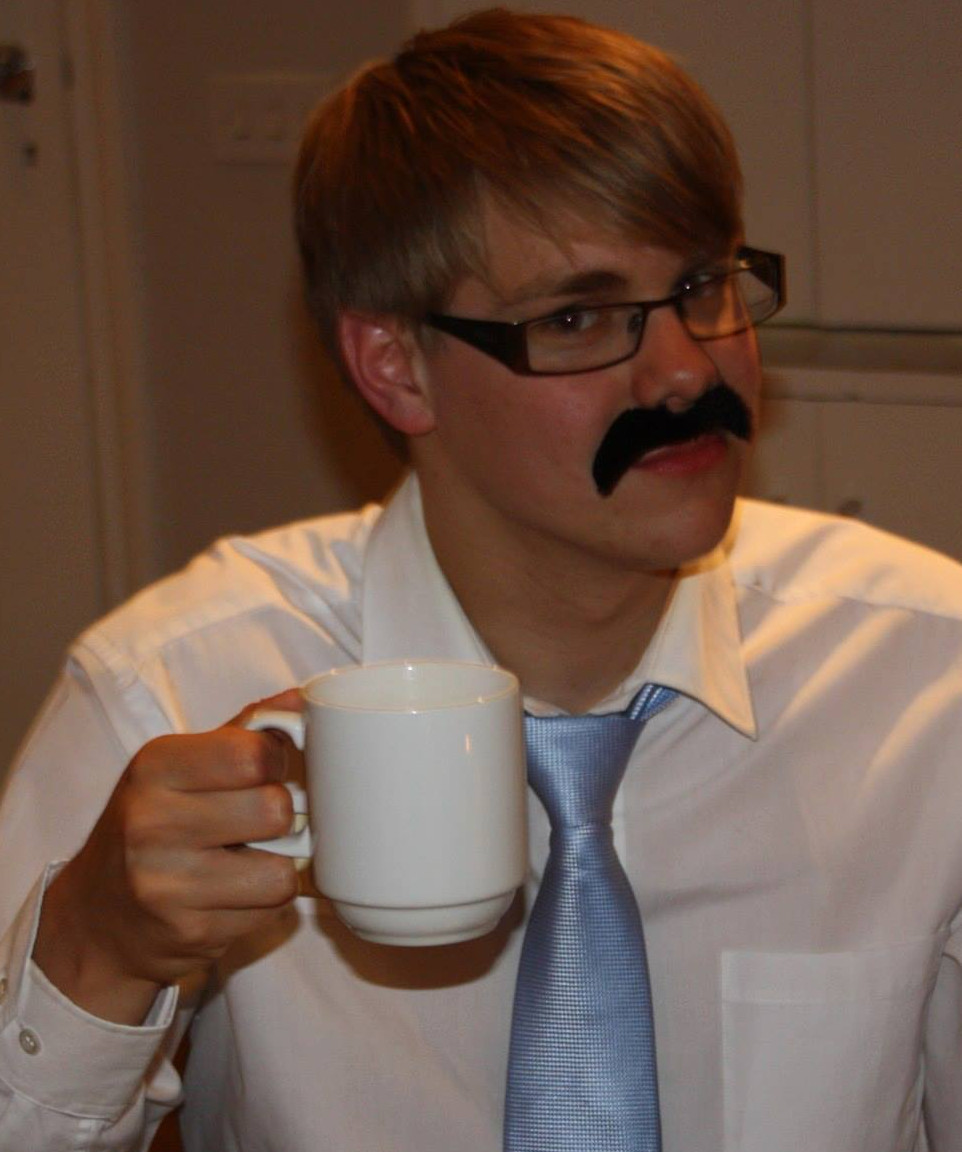
\includegraphics[width=0.8\textwidth]{AndyProfile.jpg}
\end{minipage}
\hfill
\begin{minipage}{0.6\textwidth}
  {\large \textbf{\underline{Andy Holt}}}\\

  Andy leads development of the technology side, bringing
  his information engineering background to the task of finding the
  optimal route and monitoring delays.\\

  \textbf{Subject:} Engineering (Electrical and Information)\\
  \textbf{Role:} Software monkey\\
  \textbf{Coffee time beverage:} Colombian, white
\end{minipage}

\bigskip

\noindent \begin{minipage}{0.4\textwidth}
  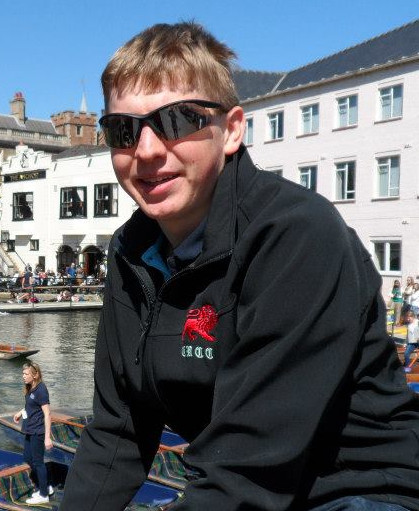
\includegraphics[width=0.8\textwidth]{ChrisProfile.jpg}
\end{minipage}
\hfill
\begin{minipage}{0.6\textwidth}
  {\large \textbf{\underline{Chris Murkin}}}\\

  Chris brings his love of optimising flow networks to the challenge
  of finding the best route. A keen cyclist, if ever cycle support is
  required, Chris will be glad to provide it.\\

  \textbf{Subject:} Chemical Engineering\\
  \textbf{Role:} Optimisation\\
  \textbf{Coffee time beverage:} Strong and black
\end{minipage}

\bigskip

\noindent \begin{minipage}{0.4\textwidth}
  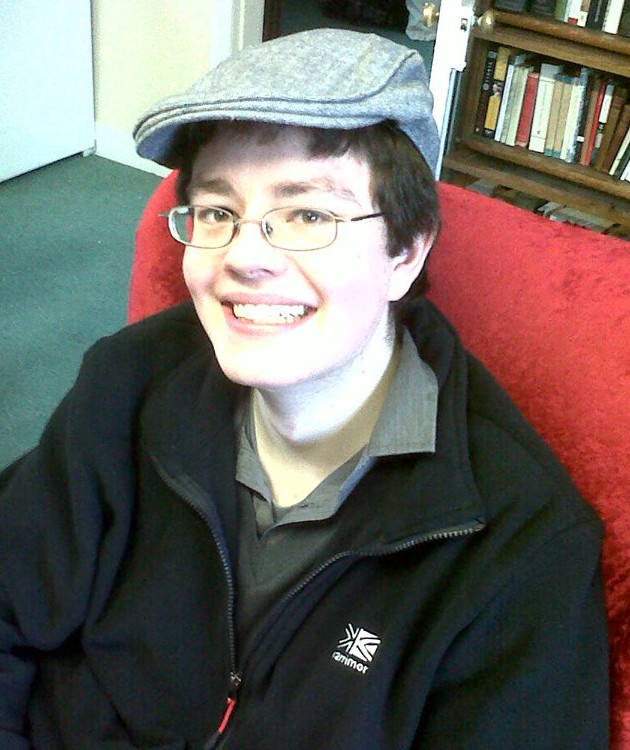
\includegraphics[width=0.8\textwidth]{DominicProfile.jpg}
\end{minipage}
\hfill
\begin{minipage}{0.6\textwidth}
  {\large \textbf{\underline{Dominic Newman}}}\\

  Dominic brings his love of railways and underground systems, as well
  as bringing a touch of sophistication to the team. A Londoner, Dominic
  also brings his inside knowledge of the tube system to bear.\\

  \textbf{Subject:} MML (French and German)\\
  \textbf{Role:} Insider knowledge\\
  \textbf{Coffee time beverage:} Tea. Of course.
\end{minipage}

\bigskip

\noindent \begin{minipage}{0.4\textwidth}
  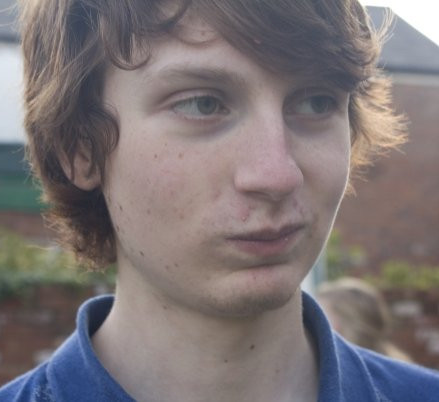
\includegraphics[width=0.8\textwidth]{JackProfile.jpg}
\end{minipage}
\hfill
\begin{minipage}{0.6\textwidth}
  {\large \textbf{\underline{Jack Robinson}}}\\

  Jack is passionate about all aspects of transport and optimisation. \\

  \textbf{Subject:} Maths, Masters in Transport Planning\\
  \textbf{Role:} Optimisation\\
  \textbf{Coffee time beverage:} Hot chocolate
\end{minipage}

\bigskip

\section*{The Strategy}

\end{document}